\section{Graph and network optimization}

\subsection{Graphs}

\subsubsection{Definitions and characteristics}

In the following section we will explain some basic concepts about the graphs. The terms used are important, and we will use the definition box to highlight these words.

\highspace
\begin{definitionbox}[: graph]
    A \definitionWithSpecificIndex{graph}{Graph} is a pair $G = \left(N,E\right)$, with $N$ a set of \textbf{nodes} or \textbf{vertices} and $E \subseteq N \times N$ a set of \textbf{edges} or \textbf{arcs} connecting them pairwise.
\end{definitionbox}

\highspace
\begin{definitionbox}[: edge]
    An \definitionWithSpecificIndex{edge}{Edge} connecting the nodes $i$ and $j$ is represented by
    \begin{itemize}
        \item Graph undirected: $\left\{i,j\right\}$
        \item Graph directed: $\left(i,j\right)$
    \end{itemize}
\end{definitionbox}

\highspace
\begin{examplebox}
    For \example{example}, a road network which connects $n$ cities can be modelled, by a graph where a city corresponds to a node, and a connection corresponds to an edge.

    \begin{center}
        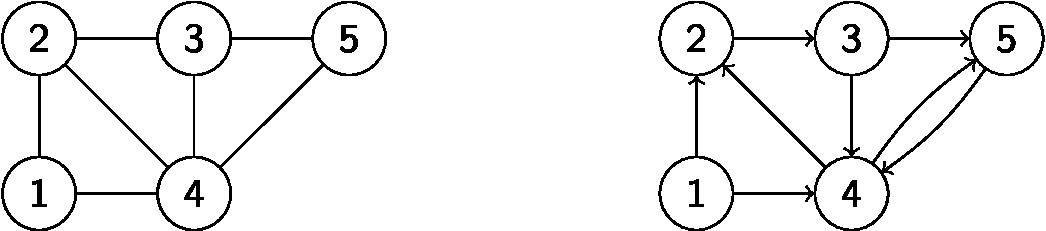
\includegraphics[width=.8\textwidth]{img/graphs-1.pdf}
    \end{center}

    \noindent
    \begin{itemize}
        \item Undirected graph:
        \begin{itemize}
            \item $N = \left\{1,2,3,4,5\right\}$
            \item $E = \left\{
                \left\{1,2\right\},
                \left\{1,4\right\},
                \left\{2,3\right\},
                \left\{2,4\right\},
                \left\{3,4\right\},
                \left\{3,5\right\},
                \left\{4,5\right\}
            \right\}$
        \end{itemize}
        
        \item Directed graph:
        \begin{itemize}
            \item $N = \left\{1,2,3,4,5\right\}$
            \item $E' = \left\{
                \left(1,2\right),
                \left(1,4\right),
                \left(2,3\right),
                \left(2,4\right),
                \left(3,4\right),
                \left(3,5\right),
                \left(4,5\right)
            \right\}$
        \end{itemize}
    \end{itemize}
\end{examplebox}

\newpage

\noindent
Some graph properties are:
\begin{itemize}
    \item Two \textbf{nodes} are \definitionWithSpecificIndex{adjacent}{Adjacent nodes} if they are \textbf{connected by an edge}.

    \item An \textbf{edge} $e$ is \definitionWithSpecificIndex{incident}{Incident edge} in a node $v$ if $v$ is an endpoint of $e$.
    
    In other words, in a graph $G$, two edges are incident \textbf{if they share a common vertex}. For example, edge $E_{1}=\left(v_{1}, v_{2}\right)$ and edge $\left(v_{1}, v_{3}\right)$ are incident as they share the same vertex $v_{1}$.

    \item The degree concept depends on the type of graph:
    \begin{itemize}
        \item Undirected graph: the \definitionWithSpecificIndex{degree}{Node degree} of a node is the \textbf{number of incident edges}.

        \item Directed graph: the \definitionWithSpecificIndex{in-degree}{Node in-degree} and \definitionWithSpecificIndex{out-degree}{Node out-degree} of a node is the \textbf{number of arcs that have it as succesor} and \textbf{predecessor}.
    \end{itemize}
\end{itemize}

\highspace
\begin{examplebox}[: adjacent, incident, degree, in-degree and out-degree]
    Given the graphs:
    
    \begin{center}
        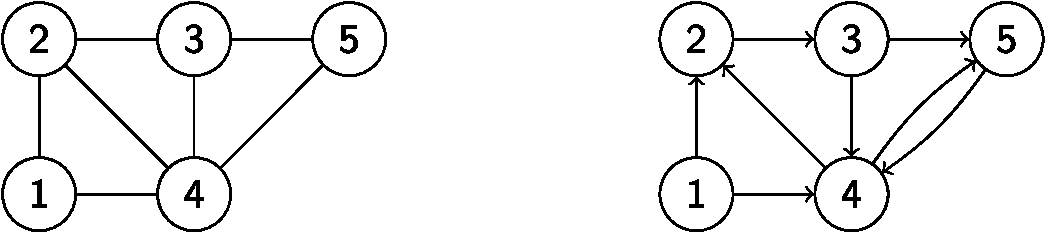
\includegraphics[width=.8\textwidth]{img/graphs-2.pdf}
    \end{center}

    \begin{itemize}
        \item Undirected graph:
        \begin{itemize}
            \item Nodes 1 and 2 are \textbf{adjacent} (unlike nodes 1 and 3).
            \item Edge $\left\{1,2\right\}$ is \textbf{incident} in nodes 1 and 2.
            \item Node 1 has \textbf{degree} 2, node 4 has \textbf{degree} 4.
        \end{itemize}

        \item Directed graph: node 1 has \textbf{in-degree} 0, and \textbf{out-degree} 2.
    \end{itemize}
\end{examplebox}

\highspace
Other useful features include:
\begin{itemize}
    \item A \definitionWithSpecificIndex{(directed) path from $i \in N$ to $j \in N$}{Directed path from $i \in N$ to $j \in N$} is a sequence of (arcs) edges:
    \begin{equation*}
        p = \left\langle \left\{v_{1}, v_{2}\right\}, \left\{v_{2}, v_{3}\right\}, \dots, \left\{v_{k-1}, v_{k}\right\} \right\rangle
    \end{equation*}
    Connecting nodes $v_{1}$ and $v_{k}$, with $\left\{v_{i}, v_{i+1}\right\} \in E$, for $i = 0, \dots, k-1$.

    \item A generic \textbf{node} $u$ and $v$ are \definitionWithSpecificIndex{connected}{Connected nodes} if there is a path connecting them.
    
    \item A \textbf{graph} $\left(N,E\right)$ is \definitionWithSpecificIndex{connected}{Connected graph} if two generic nodes $u,v$ are connected, $\forall u,v \in N$. Recall that in generic graph notation, the variable $N$ represents a set of nodes or vertices and $E$ represents a set of edges or arcs connecting them in pairs.
    
    \item A \textbf{graph} $\left(N,E\right)$ is \definitionWithSpecificIndex{strongly connected}{Strongly connected graph} if two generic nodes $u,v$ are connected by a directed path, $\forall u,v \in N$ (for any node in the set of nodes or vertices of the graph).
\end{itemize}

\highspace
\begin{examplebox}[: directed path, connected nodes, connected graph, strongly connected]
    Given the graphs:
    
    \begin{center}
        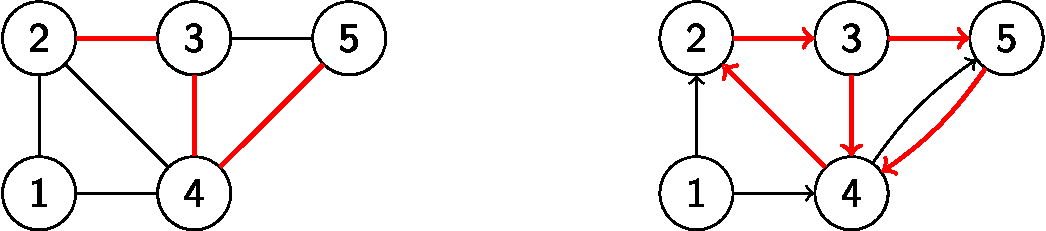
\includegraphics[width=.8\textwidth]{img/graphs-3.pdf}
    \end{center}

    \begin{itemize}
        \item Undirected graph:
        \begin{itemize}
            \item $\left\langle \left\{2,3\right\}, \left\{3,4\right\}, \left\{4,5\right\} \right\rangle$ is a \textbf{path} from node 2 to node 5.
            \item \textbf{Nodes} 2 and 5 are \textbf{connected}.
            \item It is a \textbf{connected graph}.
        \end{itemize}

        \item Directed graph:
        \begin{itemize}
            \item $\left\langle \left\{3,5\right\}, \left\{5,4\right\}, \left\{4,2\right\}, \left\{2,3\right\}, \left\{3,4\right\} \right\rangle$ is a \textbf{directed path} from node 3 to node 4.
            
            \item It is not a \textbf{strongly connected graph} because the node 1 cannot be the destination of none path. In other words, doesn't exist a directed path from node $u$ to node $1$ (where $u$ is a generic node, $\forall u \in N \setminus \left\{1\right\}$).
        \end{itemize}
    \end{itemize}
\end{examplebox}

\highspace
Finally, there are other interesting properties and notations about graphs and edges:
\begin{itemize}
    \item A \definitionWithSpecificIndex{cycle (circuit)}{Cycle in graph}\index{Circuit in graph} is a directed path with $v_{1} = v_{k}$ (source and destination are the same).

    \item A \textbf{graph} is \definitionWithSpecificIndex{bipartite}{Bipartite graph} if there is a partition $N = N_{1} \cup N_{2}$ $\left(N_{1} \cap N_{2} = \emptyset\right)$ such that no edge connects nodes in the same subset.

    \item A \textbf{graph} is \definitionWithSpecificIndex{complete}{Complete graph} if $E = \left\{\left\{v_{j}, v_{j}\right\} \: : \: v_{i}, v_{j} \in N \: \land \: i \le j\right\}$.

    \item Given a directed graph $G = \left(N,A\right)$ and $S \subset N$, the \definitionWithSpecificIndex{outgoing cut}{Outgoing cut} induced by $S$ is:
    \begin{equation*}
        \delta^{+}\left(S\right) = \left\{\left(u,v\right) \in A \: : \: u \in S \: \land : v \in N \subseteq S\right\}
    \end{equation*}
    The \definitionWithSpecificIndex{incoming cut}{Incoming cut} induced by $S$ is:
    \begin{equation*}
        \delta^{-}\left(S\right) = \left\{\left(u,v\right) \in A \: : \: v \in S \: \land : u \in N \subseteq S\right\}
    \end{equation*}
\end{itemize}

\newpage

\begin{examplebox}[: cycle/circuit in graph, bipartite graph, complete graph, out/incoming cut]
    An example of cycle in graph:
    
    \begin{center}
        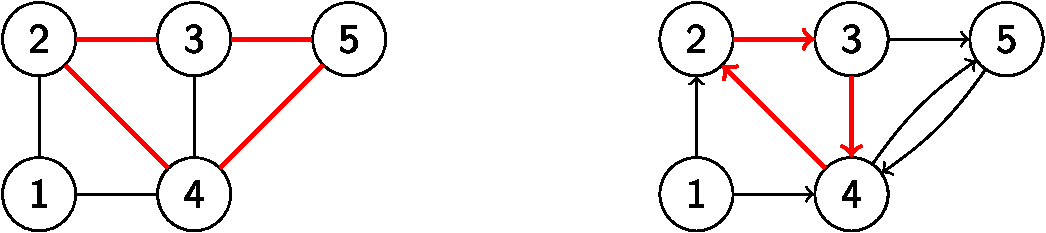
\includegraphics[width=.8\textwidth]{img/graphs-4.pdf}
    \end{center}

    \begin{itemize}
        \item Undirected graph: $\left\langle \left\{2,3\right\}, \left\{3,5\right\}, \left\{5,4\right\}, \left\{4,2\right\} \right\rangle$ is a cycle.
        \item Directed graph: $\left\langle \left(2,3\right), \left(3,4\right), \left(4,2\right) \right\rangle$ is a circuit.
    \end{itemize}
    %
    %

    An example of bipartite/complete graph:

    \begin{center}
        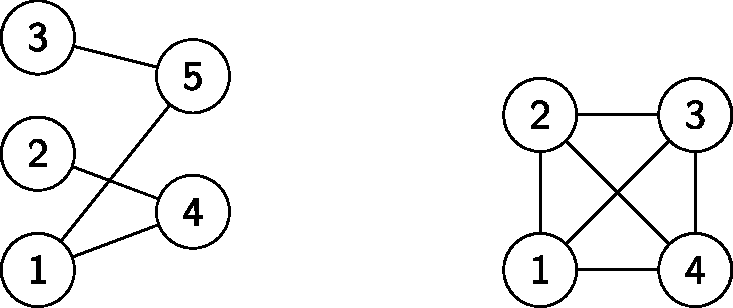
\includegraphics[width=.6\textwidth]{img/graphs-5.pdf}
    \end{center}

    \begin{itemize}
        \item To the left a \textbf{bipartite graph}, because:
        \begin{equation*}
            N_{1} = \left\{1,2,3\right\} \hspace{2em} N_{2} = \left\{4,5\right\}
        \end{equation*}
        \item And to the right a \textbf{complete graph}.
    \end{itemize}
    %
    %

    Finally, an example of out/incoming cut:
    
    \begin{center}
        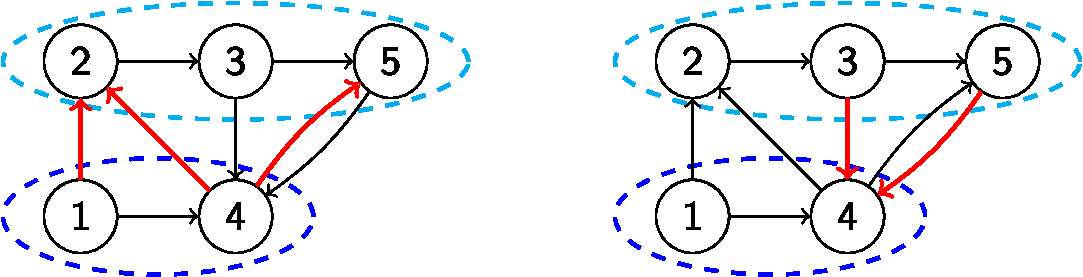
\includegraphics[width=.8\textwidth]{img/graphs-6.pdf}
    \end{center}

    \begin{itemize}
        \item Left graph: 
        \begin{equation*}
            \begin{array}{rcl}
                \delta^{+}\left(\left\{1,4\right\}\right) &=& \left(\left\{1,2\right\}, \left\{4,2\right\}, \left\{4,5\right\}\right) \\ [.5em]
                S &=& \left\{1,4\right\} \\ [.5em]
                N \setminus S &=& \left\{2,3,5\right\}
            \end{array}
        \end{equation*}

        \item Right graph: 
        \begin{equation*}
            \begin{array}{rcl}
                \delta^{-}\left(\left\{1,4\right\}\right) &=& \left(\left\{3,4\right\}, \left\{5,4\right\}\right) \\ [.5em]
                S &=& \left\{1,4\right\} \\ [.5em]
                N \setminus S &=& \left\{2,3,5\right\}
            \end{array}
        \end{equation*}
    \end{itemize}
\end{examplebox}